\chapter*{Task 3}
\addcontentsline{toc}{chapter}{Task 3}

Task 3 requires linearizing the dynamics about the generated optimal trajectory $(x^{star},u^{star})$ and using the LQR algorithm to define the optimal feedback controller to track the reference trajectory.

To compute the optimal gain for the LQR regulator, we have to solve the Linear Quadratic Optimization problem stated as follows:

\begin{equation} \label{LQR}
    \begin{aligned}
        &\min_{\Delta x \Delta u} \hspace{0.1cm} \sum_{t=0}^{T-1} \Delta x_t^TQ^{reg}\Delta x_t + \Delta u_t^TR^{reg}\Delta u_t + \Delta x_T ^TQ_T^{reg}\Delta x_T \\
        &subj. to \hspace{0.5cm} \Delta x_{t+1} = A_t \Delta x_t + B_t \Delta u_t\\
        & \hspace{2cm} \Delta x_0 = 0
    \end{aligned}
\end{equation}

The cost is already a quadratic function of the displacement states and inputs with respect to the nominal trajectory.

The LQR problem can be solved using the Difference Riccati Equation, as in (\ref{Diff ricc eq}), for the matrix $P_t$ and computing the optimal gain ${K}_t^*$. 

The task assignment requires considering an initial perturbed condition different from 0. We have selected an initial perturbation of $\delta = [0.1,0.1,0,0]^T$. In addition, we have applied noise inside the control loop.

\begin{itemize}
    \item $n_a$: It is the actuation noise. It is a normally distributed random variable with mean value 0 and variance 0.01.
    \item $n_m$: It is the measurement noise. It is a normally distributed random variable with mean value 0 and variance 0.001.
\end{itemize}

The control law applies a feedforward action, which is the optimal input obtained with Newton's method, and then uses LQR to stabilize the system.

\begin{equation}
    \begin{aligned}
        &{u}_t = {K}_t^*(x_{t+1} - x_t^{star} + n_m) + u_t^{star} + n_a\\
        &{x}_{t+1} = f_d(x_t,u_t)
    \end{aligned}
\end{equation}

The weights in the regulator cost have been selected as:

\begin{equation*}
    \begin{aligned}
        &Q_t^{reg} = \begin{bmatrix}
            1000 & 0 & 0 & 0 \\
            0 & 1000 & 0 & 0 \\
            0 & 0 & 10 & 0\\
            0 & 0 & 0 & 10
        \end{bmatrix} = Q_T^{reg}\\
        &\\
    & R^{reg}_t = 10
    \end{aligned}
\end{equation*}

As we can see from the plots, the system follows the reference, and the control loop is robust with respect to noise and a perturbed initial condition.

\begin{figure}
    \centering
    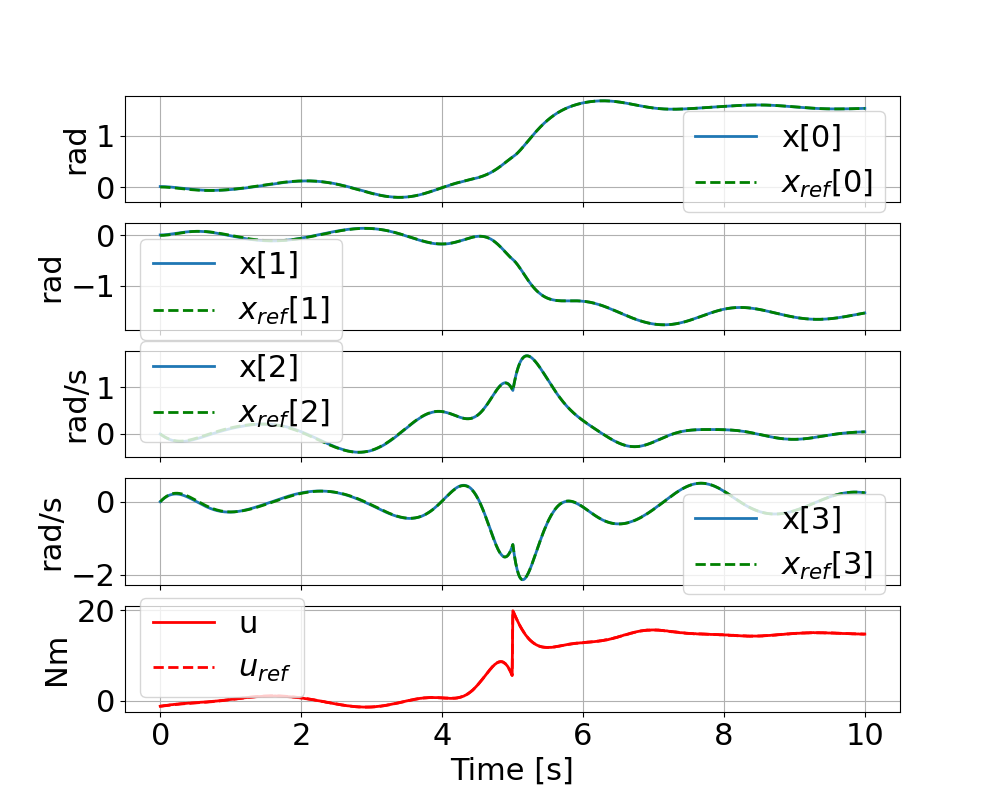
\includegraphics[width=0.8\linewidth]{figs/downward_lqr_track.png}
    \caption{Reference Tracking with LQR}
    \label{fig:downward_lqr_track}
\end{figure}

\begin{figure}
    \centering
    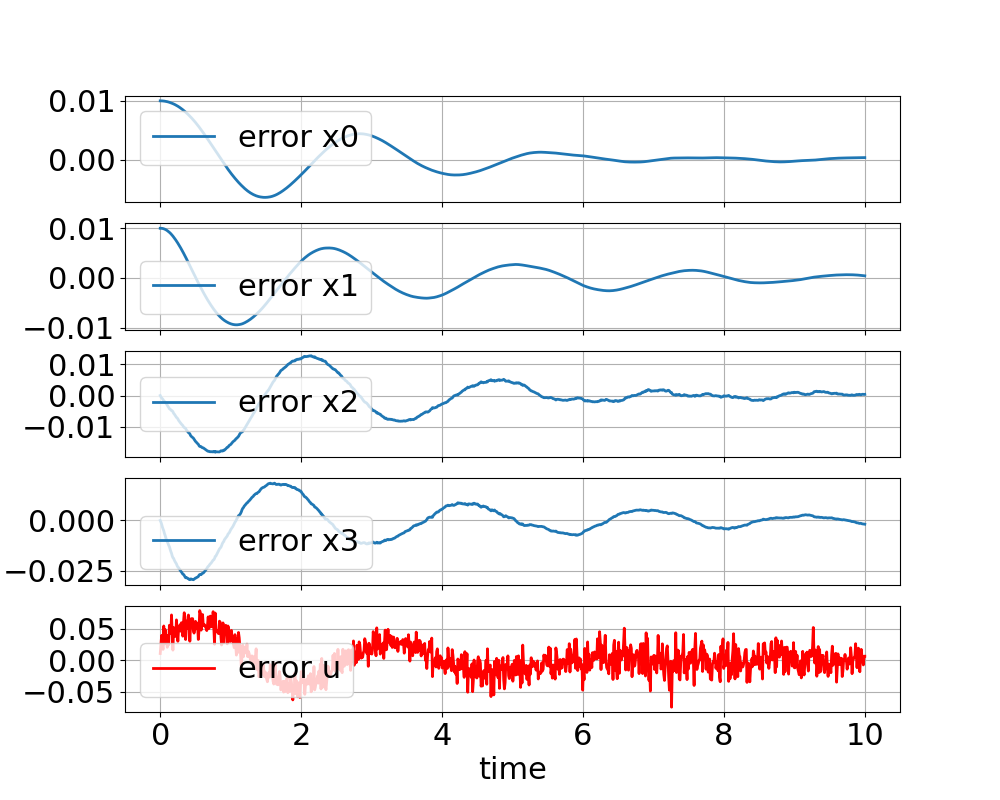
\includegraphics[width=0.8\linewidth]{figs/downward_lqr_error.png}
    \caption{Tracking error}
    \label{fig:downward_lqr_error}
\end{figure}

\begin{figure}
    \centering
    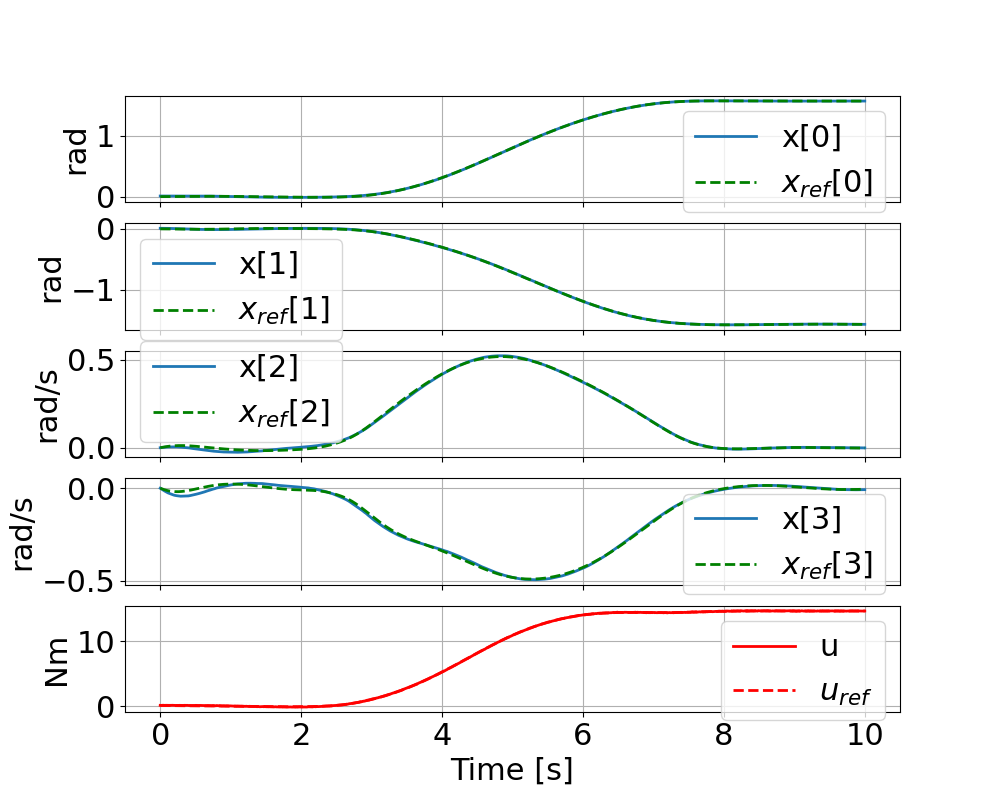
\includegraphics[width=0.8\linewidth]{figs/downward_lqr_error_smooth.png}
    \caption{Smooth reference Tracking with LQR}
    \label{fig:downward_lqr_track_smooth}
\end{figure}

\begin{figure}
    \centering
    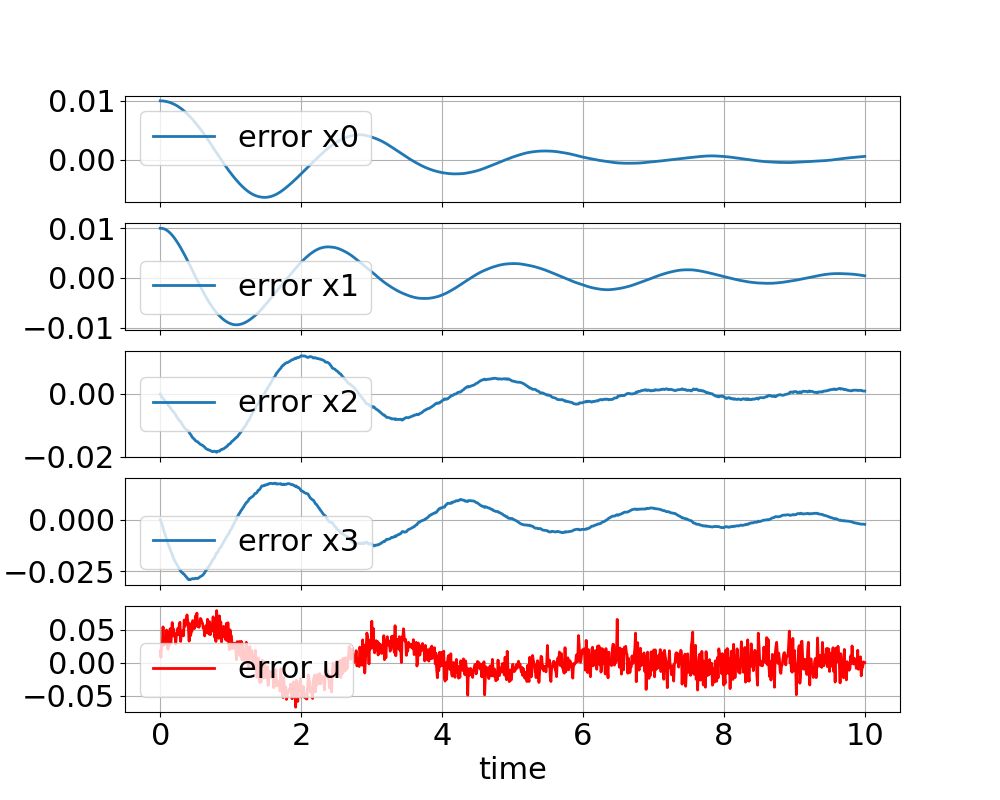
\includegraphics[width=0.8\linewidth]{figs/downward_lqr_track_smooth.png}
    \caption{Smooth reference tracking error}
    \label{fig:downward_lqr_error_smooth}
\end{figure}

\section*{Python code}

The LQR solver has been defined in the python file solver.py.

\begin{itemize}
    \item \textbf{LQR\_solver(xx\_star, uu\_star, dyn, A\_f, B\_f, QQt, RRt, tf, dt) }: Compute the optimal gain matrix $K_t^*$ for each time instant.\\\\
    \textbf{Arguments}:
    \begin{itemize}
        \item xx\_star : Optimal state reference trajectory.
        \item uu\_star : Optimal input reference trajectory.
        \item dyn : dynamic package imported from Dinamics.py.
        \item A\_f : Symbolic rappresentation of the discretized state jacobian.
        \item B\_f : Symbolic rappresentation of the discretized input jacobian.
        \item QQt : Weight matrix for the states.
        \item RRt: Weight matrix for the inputs.
        \item tf : Final simulation time, in seconds.
        \item dt : Time of dicretization in seconds.
    \end{itemize}
    \textbf{Return}:
    \begin{itemize}
        \item KK\_t : Optimal feedback gain matrix for each time instant.
    \end{itemize}
\end{itemize}